\documentclass[10pt]{article}
\usepackage[polish]{babel}
\usepackage[utf8]{inputenc}
\usepackage[T1]{fontenc}
\usepackage{amsmath}
\usepackage{amsfonts}
\usepackage{amssymb}
\usepackage[version=4]{mhchem}
\usepackage{stmaryrd}
\usepackage{graphicx}
\usepackage[export]{adjustbox}
\graphicspath{ {./images/} }

\title{XV Konkurs Matematyczny St@ś }

\author{}
\date{}


\begin{document}
\maketitle
XIV LO im. Stanisława Staszica\\
25 maja 2015 roku

\section*{klasa V}
Na rozwiqzanie poniższych zadań masz 90 minut. Kolejność rozwiazywania tych zadań jest dowolna. Wszystkie zadania sa jednakowo punktowane. Maksymalna liczbe punktów może uzyskać jedynie petne rozwiazanie, z uzasadnieniem \(\boldsymbol{i}\) odpowiedziq.\\
Używanie korektora i korzystanie z kalkulatora jest niedozwolone.

\begin{enumerate}
  \item Oblicz:
\end{enumerate}

\[
\frac{666666 \cdot 666666}{1+2+3+4+5+6+5+4+3+2+1}-\frac{777777 \cdot 777777}{1+2+3+4+5+6+7+6+5+4+3+2+1}
\]

\begin{enumerate}
  \setcounter{enumi}{1}
  \item Ile jest dziesięciocyfrowych liczb nieparzystych o sumie cyfr równej 3.
  \item Dany jest trapez równoramienny \(A B C D\) o podstawach \(A B\) i \(C D\). Na przedłużeniu boku \(A B\) poza punkt \(B\) wybrano taki punkt \(E\), że \(A C=E C\). Udowodnij, że odcinki \(B E\) i \(C D\) mają równą długość.\\
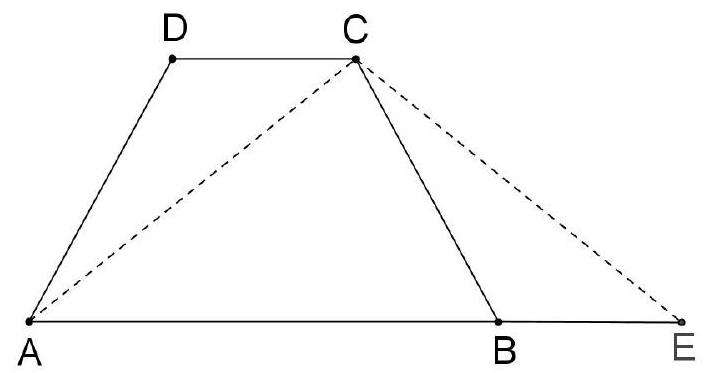
\includegraphics[max width=\textwidth, center]{2024_11_21_bddaf9af0be1a5c8781bg-1}
  \item Na przyjęcie przyszło 50 osób. Niektórzy podali sobie ręce na powitanie. Udowodnij, że liczba osób, które przywitały się z nieparzystą liczbą osób jest parzysta.
  \item Staś napisał na tablicy liczby naturalne \(1,2,3\). W jednym ruchu może zetrzeć dowolną z napisanych liczb i zamiast niej napisać liczbę będącą sumą dwóch pozostałych. Czy po pewnej liczbie takich ruchów na tablicy może pojawić się trójka liczb: 966, 1410 i 2376 ?
\end{enumerate}

\end{document}